\chapter{Корзины и мячи}
\label{ch:BucketsAndBalls}

Связанные данные по-прежнему в значительной степени неизвестны или неправильно поняты и недооценены. Часто людям это кажется слишком сложным. 
Попробуем разобраться, начнем с переменных.

Что такое переменная в SPARQL? Просто заполнитель. Но как вы можете представить себе заполнитель? Это абстрактно. У нас нет способа постичь абстрактные вещи, если мы не ассоциируем их с чем-то физическим и конкретным. Трудно представить себе время, но как только мы рисуем его в пространстве, становится легче. Мы не можем представить мебель вообще, но представить стул может каждый.

Другая трудность заключается в том, чтобы сформулировать запрос на языке SPARQL. Хотя работа со SPARQL помогает понять, как работает граф знаний, запрос SPARQL на него не похож. Это как с символами в математике. <<5 не похоже на пять, в то время как ||||| равно пяти>>. Проблема со SPARQL аналогична:

\begin{quote}
Вы хотите запросить график знаний.\\
Вы хотите узнать что-то новое.\\
Но ваш запрос не похож на граф знаний.\\
Это похоже на линии струн.\\
\end{quote}

Итак, как решить проблему с определением переменной и формулировкой SPARQL~---запроса?

Между собой представим каждый запрос SPARQL в виде графа связанных корзин и мячей.

Переменные являются заполнителями, но абстрактными. Нам нужен физический контейнер, чтобы наполнить его вещами. Нам нужны корзины. И вершины похожие на мячи. Итак, подумайте о выполнении запроса, как о заполнении корзин мячами.

Тогда образец графа будет выглядеть как на рис. ~\ref{fig:graphPattern}.

\begin{marginfigure}[-1.5cm]
	{
		\setlength{\fboxsep}{0pt}%
		\setlength{\fboxrule}{1pt}%
		\fcolorbox{gray}{gray}{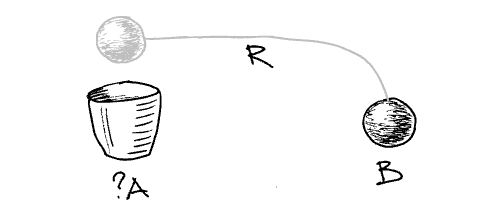
\includegraphics{./intro/bucketsAndBalls/graphPattern.PNG}}
	}
    \caption{Образец графа заполнения корзин мячами.}
	\label{fig:graphPattern}
\end{marginfigure}

Корзина \textbf{?A} должна быть заполнена теми мячами, которые имеют отношение \textbf{R} к мячу \textbf{B}.

Рисунок будет понятнее, если мы упростим его так: рис. ~\ref{fig:graphPatternBucketsBalls}: 

\begin{marginfigure}[1.0cm]
	{
		\setlength{\fboxsep}{0pt}%
		\setlength{\fboxrule}{1pt}%
		\fcolorbox{gray}{gray}{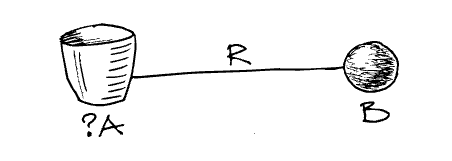
\includegraphics{./intro/bucketsAndBalls/graphPatternBucketsBalls.PNG}}
	}
    \caption{Шаблон графа в нотации <<Корзины и мячи>>.}
	\label{fig:graphPatternBucketsBalls}
\end{marginfigure}

Это шаблон графа в нотации <<Корзины и мячи>>. Направление отношения R не показано, но оно всегда слева направо.

Тогда процесс написания и выполнения SPARQL~---запроса будет состоять из шагов:
\begin{enumerate}
    \item Выберите свои корзины (в них вы собираетесь набирать нужные вам мячи).
    \item Составьте свои условия в виде графа корзин и мячей.
    \item Запустите свой запрос, чтобы заполнить ваши корзины мячами.
\end{enumerate}

Теперь напишем запрос, чтобы, например, получить всех глав правительств областей России, следуя этим шагам.

\begin{enumerate}
    \item Нам нужны две корзины, одна для регионов и одна для глав правительств.
    \item Корзина для региона должна быть привязано к мячу <<область России>> с отношением <<экземпляр>> и она должна быть связана с корзиной для <<главы правительства>>, которая, учитывая направление, следует рассматривать как <<имеет главу правительства>>, в нашем случае это будет губернатор или глава области
\end{enumerate}

Сделаем запрос более интересным и добавим еще одну корзину для фотографий губернаторов. Вот теперь запрос в нотации <<Корзины и мячи>> будет таким:

\begin{figure*}[h!]
    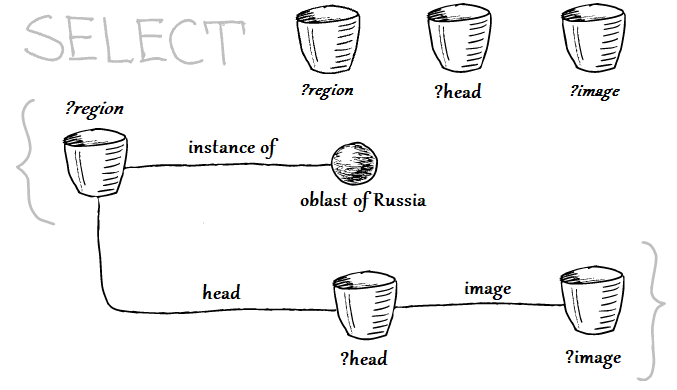
\includegraphics[width=0.7\linewidth]{./intro/bucketsAndBalls/select.PNG}
    \caption{Корзины и мячи.}
	\label{fig:BucketsBalls}
\end{figure*}

\newpage
После выполнения запроса наши корзины будут выглядеть как на рис. ~\ref{fig:BucketsBallsQuery}.

\begin{marginfigure}
	{
		\setlength{\fboxsep}{0pt}%
		\setlength{\fboxrule}{1pt}%
		\fcolorbox{gray}{gray}{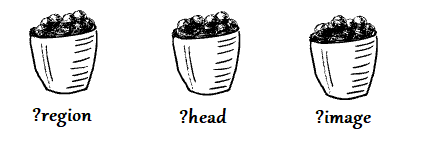
\includegraphics{./intro/bucketsAndBalls/query.PNG}}
	}
    \caption{Корзины при выполнении запроса.}
	\label{fig:BucketsBallsQuery}
\end{marginfigure}

Теперь перейдем к Викиданным и напишем этот запрос там. Сначала выберем корзины для заполнения.

\begin{lstlisting}[ language=SPARQL ]
SELECT DISTINCT ?region ?head ?image
\end{lstlisting}

Далее напишем условия соответствия мячей корзинам. Все условия в SPARQL должны заключаться в фигурные скобки {}.

Когда нам нужно определенное отношение или мяч, нам нужно использовать его идентификатор. Викиданные предоставляют хорошую услугу, которая записывает идентификатор для вас, как только вы выбираете отношение (свойство) или мяч (элемент) по его метке. Общая часть отношений в графе знаний Викиданных сокращена с помощью wdt, а элементов (наших мячей) ~--- с помощью wd.

Следуя нашему рисунку <<Корзины и мячи>> ~\ref{fig:BucketsBalls}, напишем условия для заполнения первой корзины ?region. Затем напишем первое отношение. Поскольку общей частью идентификаторов прямых отношений является wdt, мы пишем wdt:, а затем нажимаем Ctrl+пробел, чтобы запустить службу автозаполнения Викиданных рис. ~\ref{fig:BucketsBallsProperty}.

\begin{marginfigure}[-2.5cm]
	{
		\setlength{\fboxsep}{0pt}%
		\setlength{\fboxrule}{1pt}%
		\fcolorbox{gray}{gray}{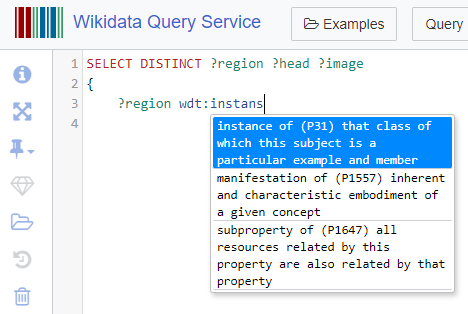
\includegraphics{./intro/bucketsAndBalls/property.PNG}}
	}
    \caption{С помощью команды Ctrl+пробел открылось выпадающее контекстное меню автозаполнения свойства Викиданых.}
	\label{fig:BucketsBallsProperty}
\end{marginfigure}

После этого мы воспроизведем модель из рисунка <<Корзины и мячи>> ~\ref{fig:BucketsBalls} в реальном запросе SPARQL.

Обычно при написании SPARQL~---запроса его приравнивают к виду таблицы с тремя столбцами: субъект, предикат, объект или на языке викиданных ~--- элемент, свойство, значение.

Но это укрепляет мышление. Поэтому, возможно, было бы лучше, чтобы хотя бы ваши первые запросы напоминали граф. Ставя корзину как субъект нового графа (тройной шаблон) под той же корзиной, которая является объектом предыдущего тройного шаблона, делает его более похожим на граф с рисунка корзины и шары ~\ref{fig:BucketsBalls}, который был представлен выше. Таким образом, наш запрос выглядит следующим образом:

\begin{lstlisting}[ language=SPARQL ]
SELECT DISTINCT ?region ?head ?image
{
    ?region wdt:P31 wd:Q835714; # oblast of Russia
    wdt:P6  ?head. # heads of government
    ?head  wdt:P18 ?image. # images of heads of government
}
\end{lstlisting}

Теперь посмотрите, как этот запрос выглядит в Викиданных, и запустите его. Затем нажмите на значок глаза слева и выберите <<image grid>>, чтобы просмотреть результаты в виде сетки изображений ~\ref{fig:BucketsBallsImageGrid}.

\begin{marginfigure}[-4.5cm]
	{
		\setlength{\fboxsep}{0pt}%
		\setlength{\fboxrule}{1pt}%
		\fcolorbox{gray}{gray}{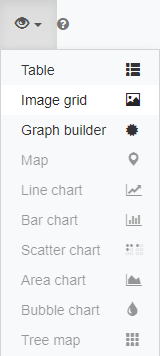
\includegraphics[width=0.5\linewidth]{./intro/bucketsAndBalls/imageGrid.PNG}}
	}
    \caption{Отображение результатов в виде сетки изображений.}
	\label{fig:BucketsBallsImageGrid}
\end{marginfigure}

Это неплохо для первого результата, но теперь на каждом изображении мы видим только идентификационные данные людей и идентификационные данные их страны. Если мы нажмем на идентификатор, мы получим много информации об этом предмете. Но было бы лучше, если бы, помимо идентификаторов, мы могли видеть их метки в результате запроса. Это похоже на наклеивание этикеток на наши корзины. 

\begin{figure*}[h!]
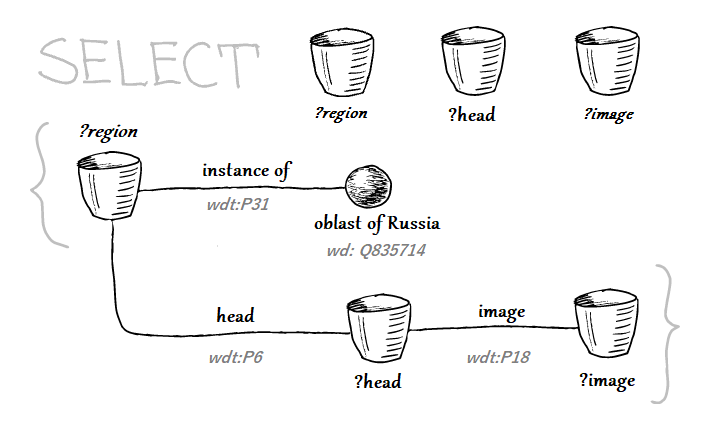
\includegraphics[width=0.6\linewidth]{./intro/bucketsAndBalls/selectID.PNG}
\caption{Корзины и мячи. Идентификаторы объектов и свойств.}
\label{fig:BucketsBallsID}
\end{figure*}

Label ~--- это метка, которая отображает название объекта(мяча), а не его идентификатор. Все, что вам нужно сделать, это: добавить слово <<label>> к переменным и вызвать службу меток. Последнее вы делаете, снова нажимая Ctrl+пробел в новой строке внутри фигурных скобок, и когда вы начнете вводить <<метку>>, появится служба маркировки. По умолчанию вы получаете его с языком интерфейса и английским языком в качестве альтернативы, если метка недоступна на языке выбранного интерфейса Викиданных.

Викиданные полны таких замечательных сервисов, и для окончательного запроса мы воспользуемся еще одним. Чтобы получить результат в сетке изображений по умолчанию, поместите где-нибудь в своем запросе следующий комментарий: \textcolor{blue}{\#defaultView:ImageGrid}

На самом деле не все нужно писать вручную. Когда вы начнете печатать, сервис автозаполнения предложит варианты.

\newpage
Наш последний запрос выглядит так (листинг~\ref{lst:regionsOfHeads}): 

\begin{lstlisting}[ language=SPARQL, caption={\href{https://w.wiki/4ENR}{Список глав областей России}\protect\footnotemark}, label=lst:regionsOfHeads, ]
# List of regions of the Russia and images of heads of government
#defaultView:ImageGrid
SELECT DISTINCT ?region ?regionLabel ?head ?headLabel ?image
{
  ?region wdt:P31 wd:Q835714; # ?region is Oblast of Russia
          wdt:P6  ?head.      #         has head of government
  ?head  wdt:P18 ?image.      # head has image
  SERVICE wikibase:label {bd:serviceParam wikibase:language "ru"} 
}
\end{lstlisting}
\footnotetext{Получено 44 области России и их глав правительства. Ссылка на SPARQL-запрос: \href{https://w.wiki/4ENR}{https://w.wiki/4ENR}}

Запустите этот скрипт.

Такое представление о запросах SPARQL как связанных корзинах и мячах может быть полезным, по крайней мере, в начале освоения Викиданных. И, конечно, у каждой метафоры есть свои ограничения. Например, нельзя поместить один и тот же мяч в две разные ностоящие корзины, но в эти виртуальные ~--- можно. <<Корзины и мячи>> могут быть полезны, чтобы вскарабкиваться на высоту абстракции Викиданных.